% Options for packages loaded elsewhere
\PassOptionsToPackage{unicode}{hyperref}
\PassOptionsToPackage{hyphens}{url}
%
\documentclass[
]{article}
\usepackage{amsmath,amssymb}
\usepackage{lmodern}
\usepackage{iftex}
\ifPDFTeX
  \usepackage[T1]{fontenc}
  \usepackage[utf8]{inputenc}
  \usepackage{textcomp} % provide euro and other symbols
\else % if luatex or xetex
  \usepackage{unicode-math}
  \defaultfontfeatures{Scale=MatchLowercase}
  \defaultfontfeatures[\rmfamily]{Ligatures=TeX,Scale=1}
\fi
% Use upquote if available, for straight quotes in verbatim environments
\IfFileExists{upquote.sty}{\usepackage{upquote}}{}
\IfFileExists{microtype.sty}{% use microtype if available
  \usepackage[]{microtype}
  \UseMicrotypeSet[protrusion]{basicmath} % disable protrusion for tt fonts
}{}
\makeatletter
\@ifundefined{KOMAClassName}{% if non-KOMA class
  \IfFileExists{parskip.sty}{%
    \usepackage{parskip}
  }{% else
    \setlength{\parindent}{0pt}
    \setlength{\parskip}{6pt plus 2pt minus 1pt}}
}{% if KOMA class
  \KOMAoptions{parskip=half}}
\makeatother
\usepackage{xcolor}
\usepackage[margin=1in]{geometry}
\usepackage{graphicx}
\makeatletter
\def\maxwidth{\ifdim\Gin@nat@width>\linewidth\linewidth\else\Gin@nat@width\fi}
\def\maxheight{\ifdim\Gin@nat@height>\textheight\textheight\else\Gin@nat@height\fi}
\makeatother
% Scale images if necessary, so that they will not overflow the page
% margins by default, and it is still possible to overwrite the defaults
% using explicit options in \includegraphics[width, height, ...]{}
\setkeys{Gin}{width=\maxwidth,height=\maxheight,keepaspectratio}
% Set default figure placement to htbp
\makeatletter
\def\fps@figure{htbp}
\makeatother
\setlength{\emergencystretch}{3em} % prevent overfull lines
\providecommand{\tightlist}{%
  \setlength{\itemsep}{0pt}\setlength{\parskip}{0pt}}
\setcounter{secnumdepth}{-\maxdimen} % remove section numbering
\ifLuaTeX
  \usepackage{selnolig}  % disable illegal ligatures
\fi
\IfFileExists{bookmark.sty}{\usepackage{bookmark}}{\usepackage{hyperref}}
\IfFileExists{xurl.sty}{\usepackage{xurl}}{} % add URL line breaks if available
\urlstyle{same} % disable monospaced font for URLs
\hypersetup{
  pdftitle={Ejercicio 13},
  pdfauthor={Jota},
  hidelinks,
  pdfcreator={LaTeX via pandoc}}

\title{Ejercicio 13}
\author{Jota}
\date{2023-02-28}

\begin{document}
\maketitle

\hypertarget{ejercicio}{%
\subsection{Ejercicio}\label{ejercicio}}

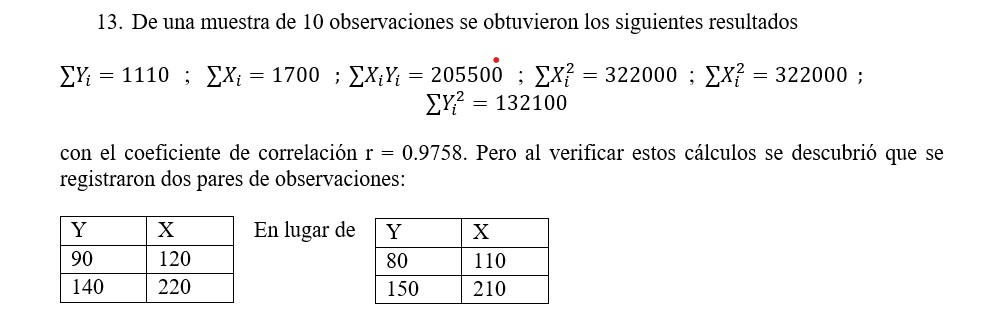
\includegraphics{13.jpg}

\hypertarget{soluciuxf3n}{%
\section{Solución}\label{soluciuxf3n}}

Primero, calculemos la correlación utilizando los datos originales:

Primero, debemos ajustar los valores de la muestra para eliminar los
errores en la grabación de datos:

\[\begin{align*}
\sum Y_i &= 1110 - 90 - 140 + 80 + 150 \\
&= 1110 - 50 \\
&= 1060 \\
\sum X_i &= 1700 - 120 - 220 + 110 + 210 \\
&= 1700 - 20 \\
&= 1680 \\
\sum X_iY_i &= 205500 - (90)(120) - (140)(220) + (80)(110) + (150)(210) \\
&= 205500 - 31800 - 30800 + 8800 + 31500 \\
&= 199200 \\
\sum X_i^2 &= 322000 - 120^2 - 220^2 + 110^2 + 210^2 \\
&= 322000 - 54400 - 48400 + 12100 + 44100 \\
&= 322000 - 46500 \\
&= 275500 \\
\sum Y_i^2 &= 132100 - 90^2 - 140^2 + 80^2 + 150^2 \\
&= 132100 - 8100 - 19600 + 6400 + 22500 \\
&= 132100 - 15300 \\
&= 116800 \\
\end{align*}\]

La nueva suma de las \(Y_i\) es de 1060, y la nueva suma de las \(X_i\)
es de 1680. Ahora podemos calcular la correlación correcta:

Donde \(\overline{X} = \frac{1}{10}\sum X_i = 170\),
\(\overline{Y} = \frac{1}{10}\sum Y_i = 111\), y se utilizó la fórmula
estándar para la correlación de Pearson.

Ahora, debemos calcular la correlación con los datos corregidos. Para
hacer esto, reemplazamos las dos observaciones incorrectas con las
observaciones correctas y recalculamos las sumas y la correlación:

\[\sum Y_i = 1110 - 90 + 80 = 1100\]

\[\sum X_i = 1700 - 120 + 110 = 1690\]

\[\sum X_iY_i = 205500 - 90 \times 120 + 80 \times 110 = 203500\]

\[\sum X_i^2 = 322000 - 120^2 + 110^2 = 318900\]

\[\sum Y_i^2 = 132100 - 90^2 + 80^2 = 131900\]

\end{document}
